
\section{Background and Motivation}
\subsection{Background}
In this work, we consider two commonly used model compression techniques, described as follows.

\cparagraph{Pruning.} This technique removes less important parameters from a trained network. Pruning ranks the neurons in the network
according how much the neuron contribute, it then removes the low ranking neurons to reduce the model size. Care must be taken to not
remove too many neurons to significantly damage the accuracy of the network.

\cparagraph{Data quantization.} This technique reduces the number of bits used to store the weights of a network, e.g., using 8-bit to
represent a 32-bit floating point number. In this work, we apply data quantization to convert a pre-trained floating point model into a
fixed point model without re-training. We choose to use an 8-bit representation as it is the most common fixed point data quantization
approach~\FIXME{\cite{}}.

\begin{figure*}[!t]
\centering
\subfloat[][Model size]{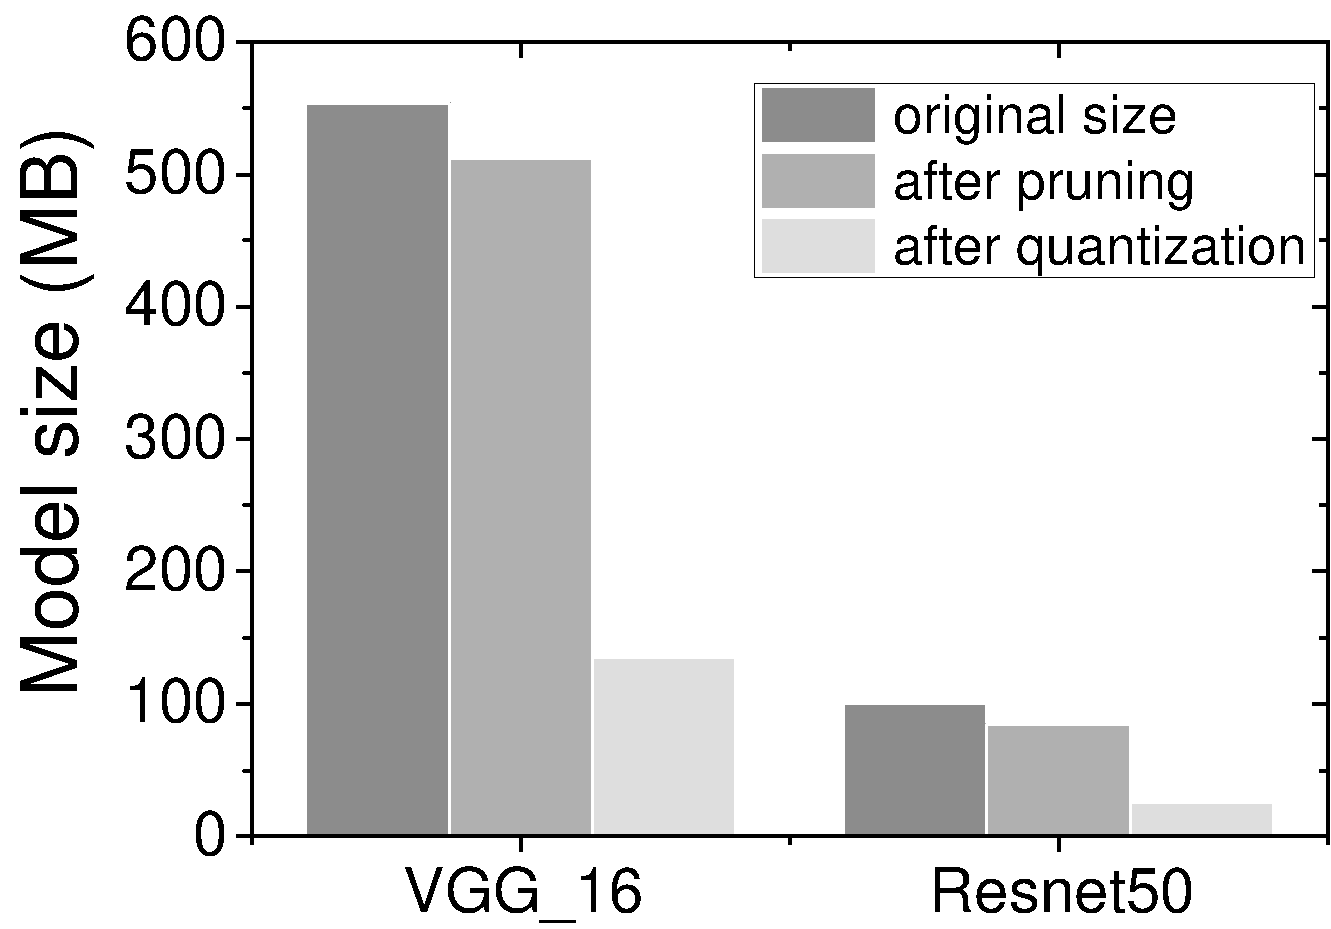
\includegraphics[width=0.28\textwidth]{figure/motivation_size.pdf}}
\hfill
\subfloat[][Inference time]{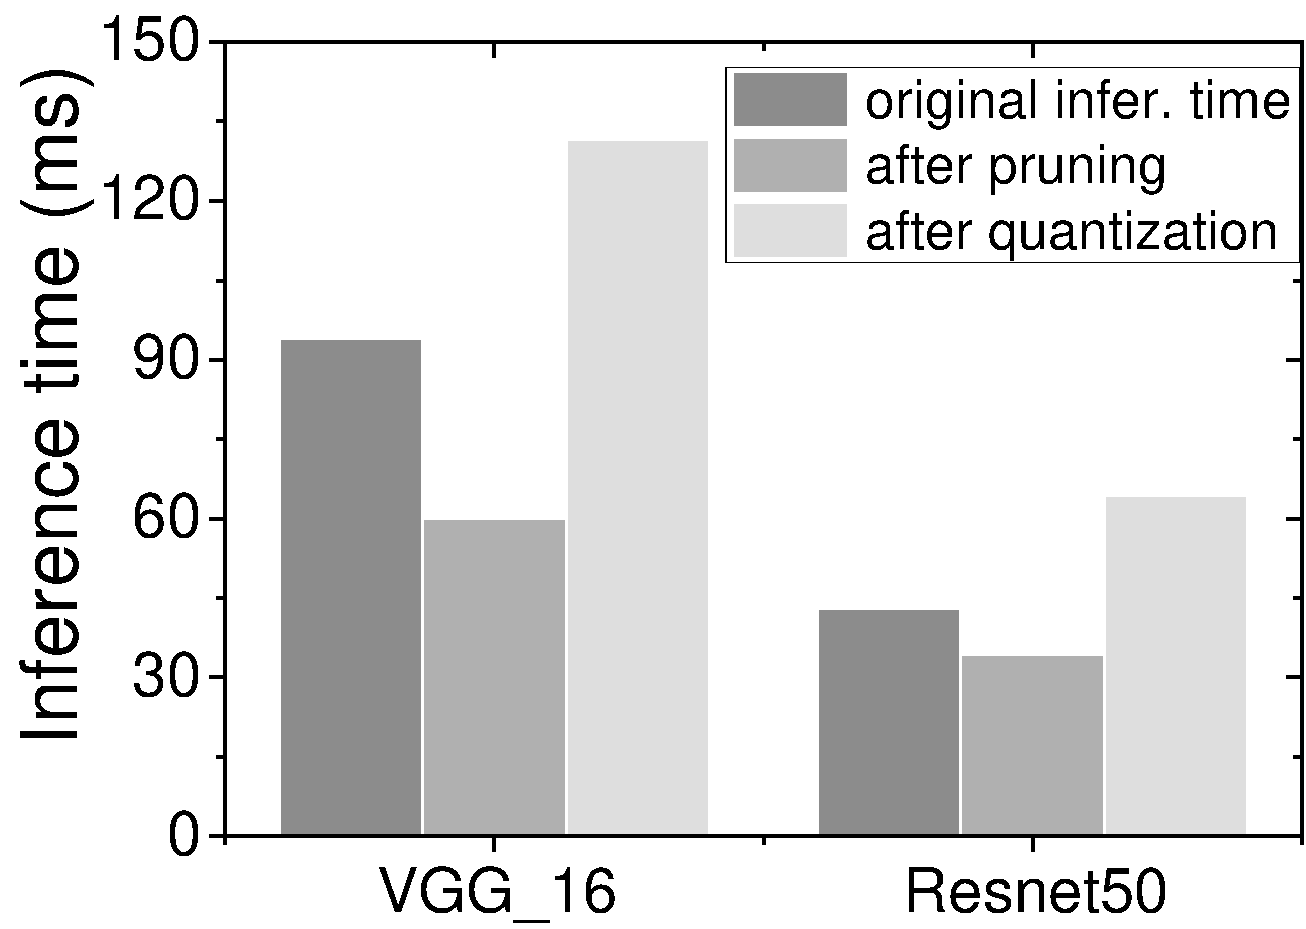
\includegraphics[width=0.28\textwidth]{figure/motivation_time.pdf}}
\hfill
\subfloat[][Accuracy]{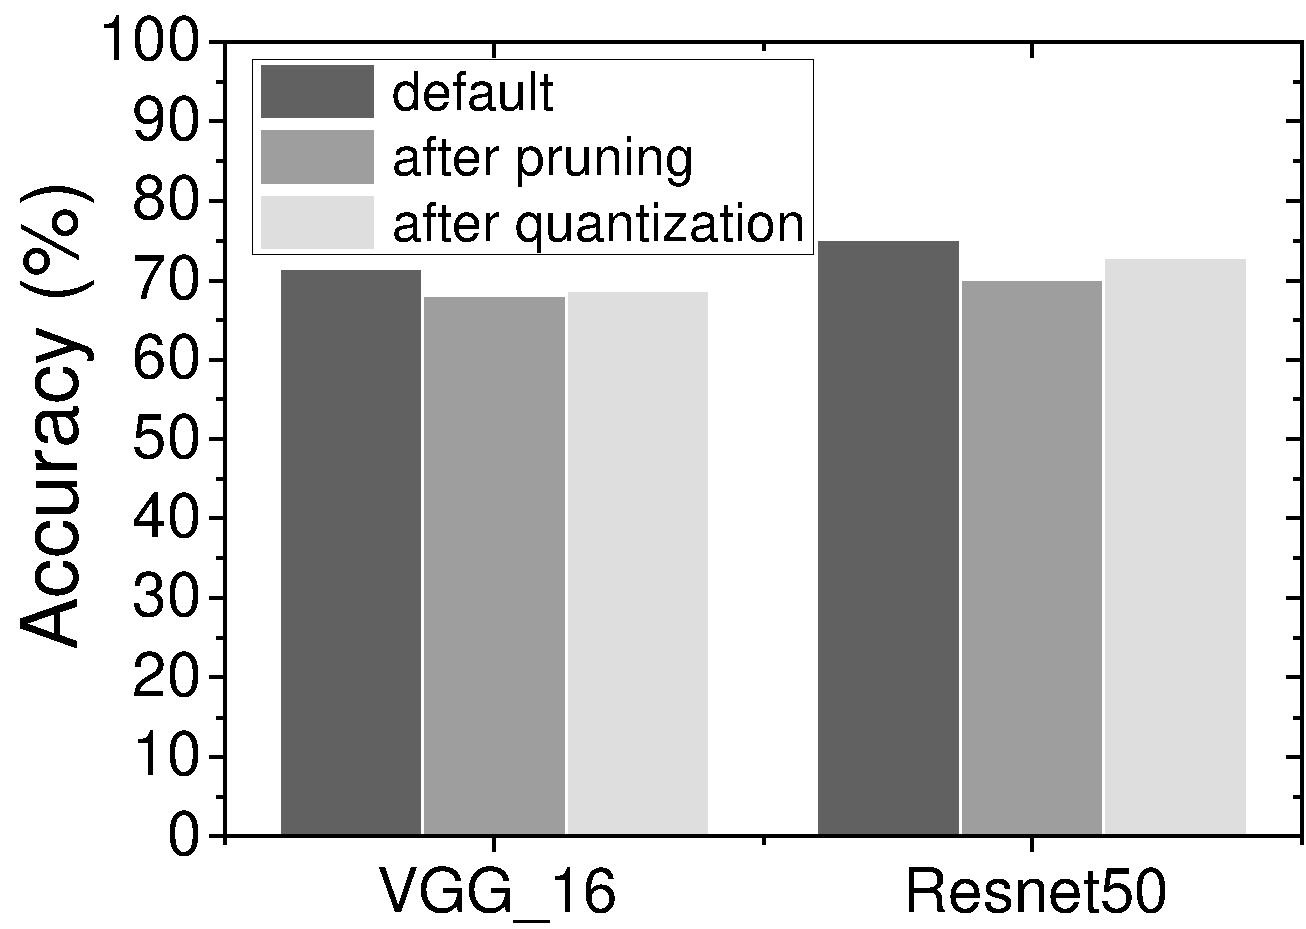
\includegraphics[width=0.28\textwidth]{figure/motivation_accuracy.pdf}}
\caption{The achieved model size (a) inference time (b) and accuracy (c) before and after the compression by \quantization and \pruning.
The compression technique to use depends on the optimization target.}
\label{fig:motivation}
\end{figure*}

\subsection{Motivation}
Choosing the right compression technique is non-trivial. As a motivation example, consider applying two widely used model compression
techniques, \pruning~\cite{manessi2017automated} and \dquantization~\cite{han2015deep}, to two influential \CNN models, \texttt{VGG\_16} 	and
\texttt{Resnet\_50}. Our evaluation platform is a NVIDIA Jetson TX2 embedded deep learning platform (see Section~\ref{sec:platform}).

\cparagraph{Setup.} We apply the compression technique to the pre-trained model (which has been trained on the ImageNet ILSVRC 2012
training dataset~\cite{imagenet2012}). We then test the original and the compressed models on ILVRSC 2012 validation set which contains 50k images.
We use pruning and quantization to compress two typical models \texttt{VGG\_16} and \texttt{Resnet 50},
and the loss of accuracy for pruning and quantization are less than 5\%,and 3\% respectively.
We use the GPU for
inferencing.

\cparagraph{Motivation Results.} Figure~\ref{fig:motivation} compares the model size, inference time and accuracy after applying model
compression. By removing some of the pathways of the network, \pruning is able to reduces the inference time by 28\%. However, it offers
little saving in storage size because network weights still deaminate the model size. By contrast, by using a few number of bits to
represent the weights, \quantization significantly reduces the model storage size by 75\%. However, the reduction in the model size does
not translate to faster inference time; on the contrary, the inference time increases by 1.45x. This is because the sparsity in network
weights brought by \quantization leads to irregular computation which causes poor GPU performance~\cite{}. Applying both compression
techniques has modest impact on the prediction accuracy, on average, less than 5\%. This suggests that both techniques can be profitable.

\cparagraph{Lessons Learned.} This example shows that the compression technique to use depends on what to be optimized for. If storage
space (e.g., RAM and disk) is a limiting factor, \quantization could be used, but a more powerful processor unit is required to achieve
quick on-device inference. If faster on-device turnaround time is a priority, \pruning can be employed but it would require sufficient
memory resources to store the model parameters.  Since offloading the computation into the cloud is often infeasible due to privacy
concerns, high latency, or the lack of connectivity, there is a need to understand the pros and cons of model compression techniques for
embedded deep learning. This work provides an extensive study to characterize the benefit and cost of commonly used deep learning
compression techniques on embedded systems.
